\documentclass{article}
\usepackage{caption, float, graphicx, subcaption}
\usepackage[dvipsnames]{xcolor}
\captionsetup[table]{skip=1em}

\title{ESE 326: Final Project}
\author{Eric Stewart \& Gabriel Minton}
\date{November 2024}


\begin{document}

\maketitle
\tableofcontents

\color{red}
\vskip 1em
!!! All content must end on page 6 !!!
\color{black}

\newpage

\section{Introduction}
The main objective of this project involoved R's built-in dataset, Iris. This dataset contains measurements of 150 iris flowers, from three species: Setosa, Versicolor, and Virginica. Each specimen has measurements of petal length, petal width, sepal length, and sepal width. Through
graphical exploration and mathematical analysis, the reseachers determine whether
there are clear rules as to which of these features can determine the species of a
given specimen. Through these two forms of analysis, the researchers will show if and how the three species of iris flowers can be differentiated by the four features.


\section{Methods}

\subsection{Exploratory Analysis}
% explain how to do analysis and what it will show 
%Section 2: Methods (general description on the methods used to carry out exploratory data
%analysis, confidence interval estimate, and hypothesis test).
%Section 3: Results and Observations (present the results obtained in the form of tables and
%figures)

Exploratory data analysis is meant for betterunderstanding and visualizing the data. This will also allow for researchers to form hypotheses and find patterns. Later in this report, these patterns will be proven or disproven given the evidence found from the mathematical Inference analysis.

For this project, the researchers have created multiple graphs showing how the features of the Iris dataset are separated between species. The first set of graphs, Figure~\ref{fig:iris_colored}, plots pairs of features separated by species. These plots begin to show separation between the features of the different species. This is not enough data to concretely show that there exist statistical differences between the features of each species. Next, the researchers created boxplots for each feature. These, shown in Figure~\ref{fig:feature_boxplots}, more discretely show separation between the three Iris species. These findings will be discussed further in the following sections.


\subsection{Confidence Interval Estimate}



\subsection{Hypothesis Test}

$\gamma$ was found through Equation~\ref{eq:gamma_unequal}.


$\sigma_1 == \sigma_2$ T-test using Sp:
\begin{equation}
	\frac{(\bar{X}_1 - \bar{X}_2) - (\mu_1 - \mu_2)}{\sqrt{{S_p}^2
	\left(\frac{1}{n_1} + \frac{1}{n_2} \right)}} \sim T_{n_1 + n_2 -2}
	\label{eq:t-test_equal}
\end{equation}
\begin{equation}
	{S_p}^2 = \frac{(n_1 - 1) S_1^2 + (n_2 -1) S_2^2}{n_1 + n_2 -2}
	\label{eq:pool_sample_variance}
\end{equation}

\noindent $\sigma_1 \neq \sigma_2$ T-test using $\gamma$:
\begin{equation}
	\frac{(\bar{X}_1 - \bar{X}_2) - (\mu_1 - \mu_2)}{\sqrt{\frac{S_1^2}{n_1} +
	\frac{S_2^2}{n_2}}} \sim T_\gamma
	\label{eq:t-test_unequal}
\end{equation}
\begin{equation}
	\gamma = \frac{\left(\frac{S_1^2}{n_1} + \frac{S_2^2}{n_2}
	\right)^2}{\frac{\left(\frac{S_1^2}{n_1} \right)^2}{n_1 - 1} +
	\frac{\left(\frac{S_2^2}{n_2} \right)^2}{n_2 - 1}}
	\label{eq:gamma_unequal}
\end{equation}


\section{Results and Observations}
\subsection{Exploratory Analysis}

Figure~\ref{fig:feature_boxplots} depicts the 6 pairings of the four features. These features are petal length, petal width, sepal length, and sepal width. Several images are jumbled together, showing that the species have no statistical difference for that feature. For example, take the Sepal Length column. There is not a distinct horizontal separation between the colored species. This means that the sepal length is roughly the same for each species of iris. Similarly, the Sepal Width column shows that there is not a significant statistical separation between species for that feature.
The Petal Length subplots show that Versicolor and Virginica are close, but the Setosa points have much smaller values. This could mean that Setosa is statistically smaller than the other two species. This is supported by Figure~\ref{fig:box_petal_length}. Likewise, the Petal Width subplots show the Versicolor and Virginica points very close, though perhaps still statistically different. The Setosa plots definitely have smaller values than those of the Versicolor and Virginica datapoints. The best plot to see these differences is the Petal Length/ Petal Width plot(s), as the blue setosa group is away from the green and red Versicolor and Virginica groups.

The researchers also prepared a set of boxplots (Figure~\ref{fig:feature_boxplots}). As a property of boxplots, the vertical separation represents a statistical difference between samples. Figures~\ref{fig:box_petal_length}~and~\ref{fig:box_petal_width} show a significant amount of difference between the species for Petal Lengths and Petal Widths, respectively. For each of these features, there is a clear separation of the species. Setosa has the smallest petals, with Versicolor and Virginica being larger. As expected, this is the same result as found from Figure~\ref{fig:iris_colored}. The boxes for Sepal Length show the same pattern, though the Versicolor and Virginica boxes have some overlap (Figure~\ref{fig:box_sepal_length}). Figure~\ref{fig_box_sepal_width} changes the previous pattern of Setosa having the smallest features. This subplot also has overlap for all three boxes, meaning there is no statistical difference between species for sepal width. This is reflected in the Sepal Width column of Figure~\ref{fig:iris_colored}, where all three species populate the same horizontal region.


\begin{figure}[h]
	\centering
	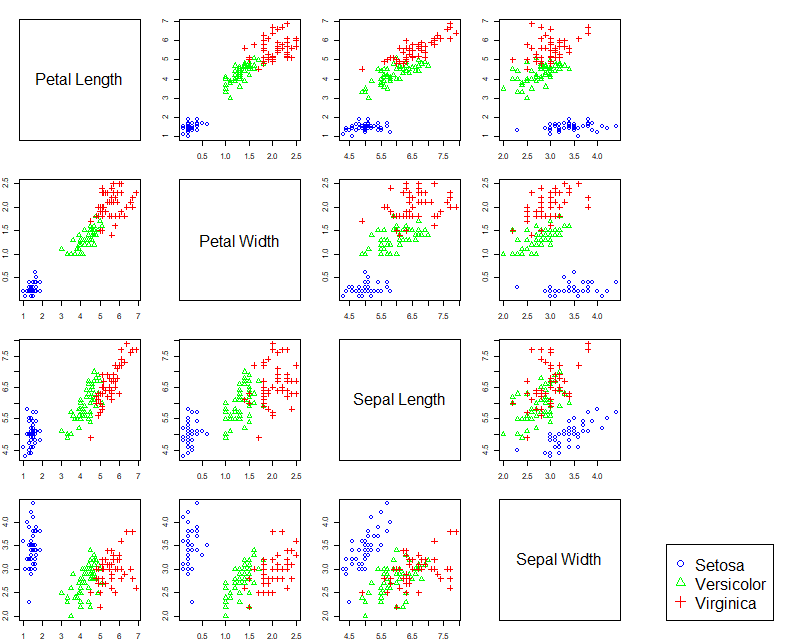
\includegraphics[width=0.75\textwidth]{iris_colored.png}
	\caption{A visualization of the Iris dataset showing scatterplots of each pair
	of the features.}
	\label{fig:iris_colored}
\end{figure}

% Show the feature boxplots together
\begin{figure}[h]
	\centering
	\begin{subfigure}{0.375\textwidth}
		\centering
		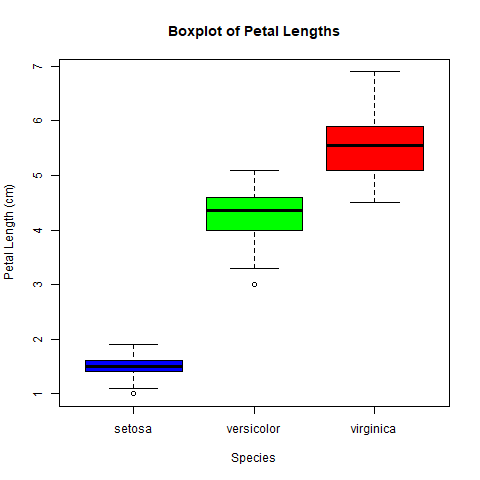
\includegraphics[width=\linewidth]{box_petal_length.png}
		\caption{Petal Lengths}
		\label{fig:box_petal_length}
	\end{subfigure}%
	\begin{subfigure}{0.375\textwidth}
		\centering
		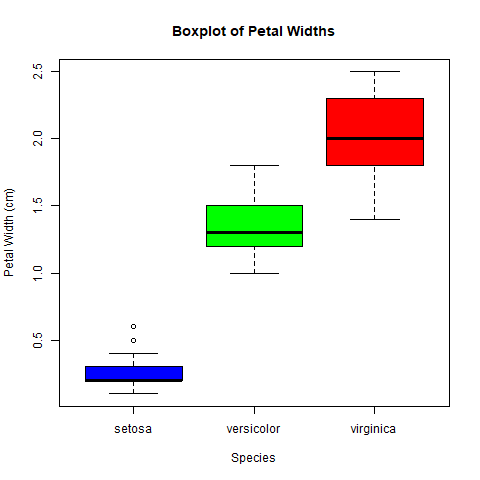
\includegraphics[width=\linewidth]{box_petal_width.png}
		\caption{Petal Widths}
		\label{fig:box_petal_width}
	\end{subfigure}\\
	\begin{subfigure}{0.375\textwidth}
		\centering
		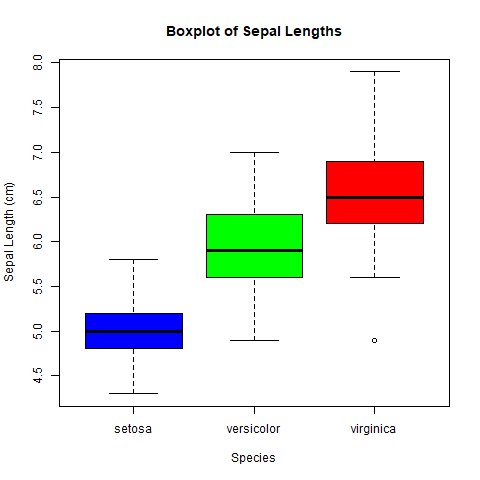
\includegraphics[width=\linewidth]{box_sepal_length.png}
		\caption{Sepal Lengths}
		\label{fig:box_sepal_length}
	\end{subfigure}
	\begin{subfigure}{0.375\textwidth}
		\centering
		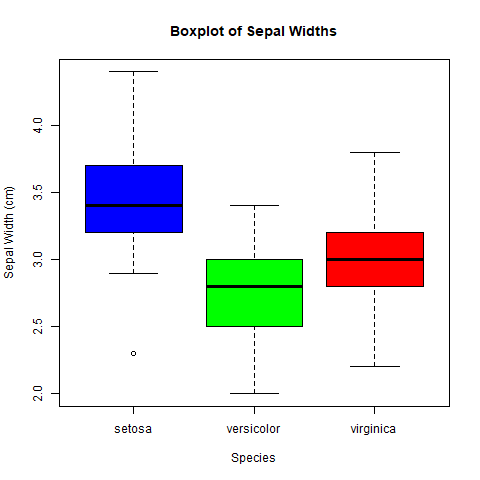
\includegraphics[width=\linewidth]{box_sepal_width.png}
		\caption{Sepal Widths}
		\label{fig:box_sepal_width}
	\end{subfigure}\\
	\caption{Boxplots for each of the four features.}
	\label{fig:feature_boxplots}
\end{figure}


\color{teal}
\subsection{Inference Analysis}

% Show the histogram plot
\begin{figure}[H]
	\centering
	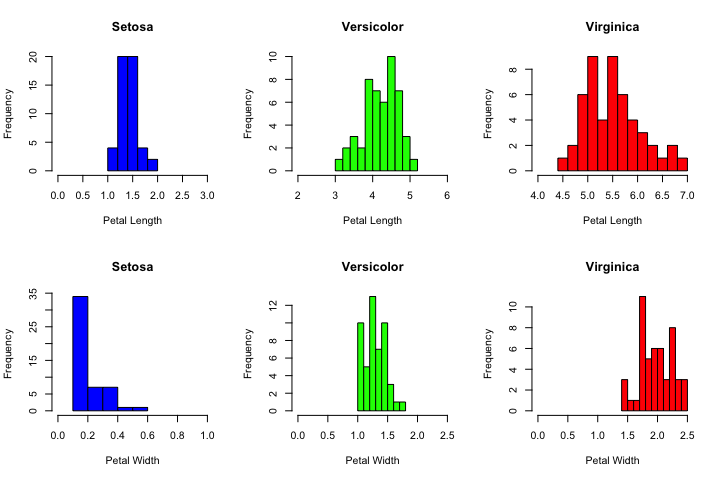
\includegraphics[width=0.75\textwidth]{hist_iris.png}
	\caption{Histograms of Petal lengths and widths for Setosa, Versicolor, and
	Virginica}
	\label{fig:hist_iris}
\end{figure}

\section{Conclusions}

\newpage
\section{Appendix}

\subsection{Extra Figures and Tables} 
\subsection{R-scripts}
\subsubsection{Exploratory.r}

contents of file...

..

..

..

\subsubsection{Inference.r}


\end{document}
